\section{Lower Voltage}
\subsubsection*{Settings}
Used settings:  \\
$f = 6.0$ Hz,  \\
Amplitude: 2.3 V,  \\
Offset: -120 mV.  \\
Filename: \texttt{ALL0003.CSV}.  

\subsection{Full Trace}

\begin{figure}[H]
    \centering
    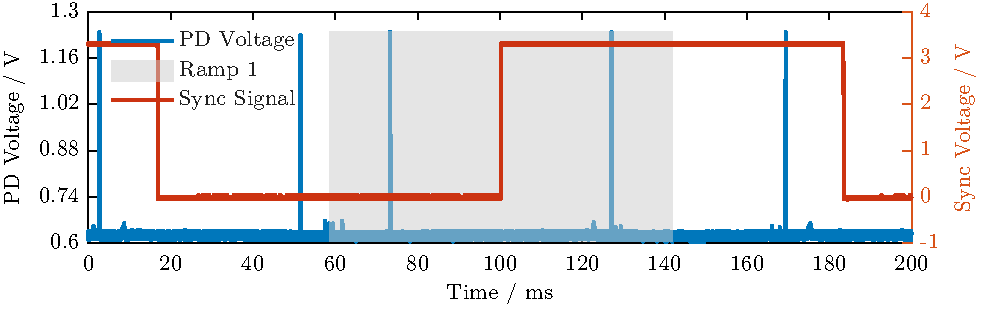
\includegraphics[width=\textwidth]{Figure_1_low.pdf}
    \caption{The rectangular signal is the sync signal of the function generator. The shaded region marks one ramp of the piezo (either increasing or decreasing the cavity length).}
    \label{fig:full_low}
\end{figure}

\subsection{Considered Region}
same as previous
\begin{figure}[H]
    \centering
    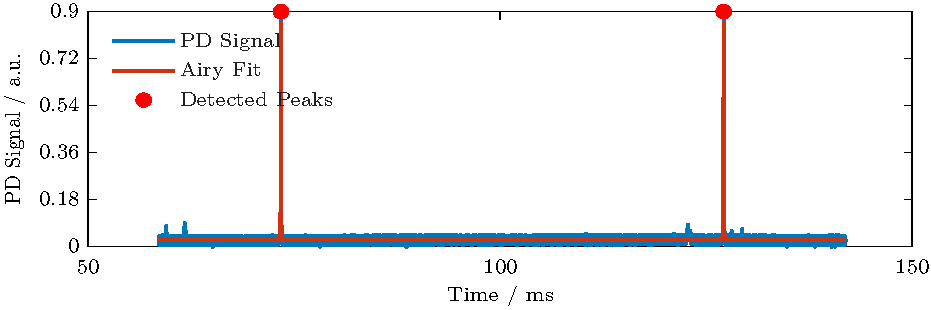
\includegraphics[width=0.9\textwidth]{Figure_2_low.pdf}
    \caption{The two detected peaks lie directly underneath the fitted Airy function. The right-most peak is not well fitted, most likely due to non-linearity of the piezo scan.}
    \label{fig:fit_low}
\end{figure}

\newpage
\subsection{Individual Peaks}
The plotted finesse is once again $\mathcal{F}=2000$.

\begin{figure}[H]
    \centering
    \begin{subfigure}[t]{0.48\textwidth}
        \centering
        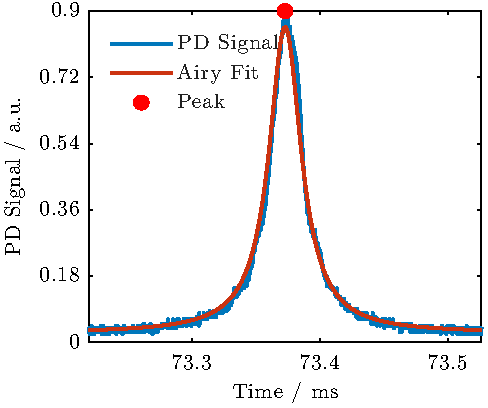
\includegraphics[width=\textwidth]{Figure_3_low.pdf}
        \caption{Zoomed-in view of Peak 1.}
        \label{fig:peak1_low}
    \end{subfigure}
    \hfill
    \begin{subfigure}[t]{0.48\textwidth}
        \centering
        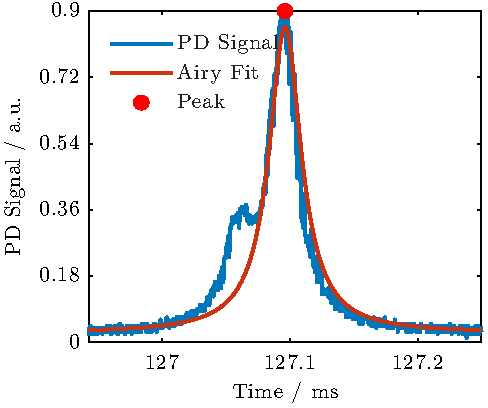
\includegraphics[width=\textwidth]{Figure_4_low.pdf}
        \caption{Zoomed-in view of Peak 2.}
        \label{fig:peak2_low}
    \end{subfigure}
    \caption{Zoomed-in views of the detected peaks in the lower-voltage scan.}
\end{figure}
